\documentclass[11pt]{article}
\usepackage{amsmath,amssymb,amsthm}
\usepackage{graphicx}
\usepackage{booktabs}
\usepackage{subcaption}
\usepackage[numbers]{natbib}
\usepackage{hyperref}
\graphicspath{{figures/}}

\newcommand{\R}{\mathbb{R}}
\newcommand{\norm}[1]{\left\lVert #1 \right\rVert}
\DeclareMathOperator*{\argmin}{arg\,min}
\newtheorem{theorem}{Theorem}
\newtheorem{lemma}[theorem]{Lemma}

\title{A Visual Tour of \LaTeX{} Rendering}
\author{Ada Lovelace\thanks{Analytical Engine Lab.} \and Alan Turing}
\date{October 2026}

\begin{document}
\maketitle

\begin{abstract}
We demonstrate inline rendering of text, equations, tables, figures and
cross-references. Everything you see is live: click a block to edit it.
\end{abstract}

\section{Introduction}\label{sec:intro}
Special relativity~\cite{einstein1905} gave us $E = mc^2$, while
\citet{knuth1984} gave us \TeX{}. Modern models~\cite{vaswani2017,knuth1984}
rely on \emph{attention}. See Section~\ref{sec:method} for details, and
\textbf{bold}, \textit{italic}, \texttt{monospace} and ``quoted'' text --- all
rendered inline.\footnote{Footnotes are shown below their paragraph.}

\section{Method}
\label{sec:method}
We minimise a regularised loss over $\theta \in \R^d$:
\begin{equation}
  \hat\theta = \argmin_{\theta} \; \frac{1}{n}\sum_{i=1}^{n} \ell(y_i, f_\theta(x_i)) + \lambda \norm{\theta}_2^2 .
  \label{eq:loss}
\end{equation}
where $\lambda > 0$. The gradient update is given by
\begin{align}
  g_t &= \nabla_\theta \mathcal{L}(\theta_t), \label{eq:grad}\\
  \theta_{t+1} &= \theta_t - \eta\, g_t. \nonumber
\end{align}
Equation~\eqref{eq:loss} and \eqref{eq:grad} are numbered automatically.

\begin{theorem}[Convergence]\label{thm:conv}
If $\ell$ is convex and $\eta < 1/L$, then $\mathcal{L}(\theta_t) \to \mathcal{L}(\hat\theta)$.
\end{theorem}

\begin{proof}
Standard; see \cite{knuth1984}.
\end{proof}

\subsection{Results}
Table~\ref{tab:results} summarises results; Figure~\ref{fig:signal} shows the
signal and Figure~\ref{fig:pair} compares two views.

\begin{table}[htbp]
  \centering
  \caption{Accuracy by method.}
  \label{tab:results}
  \begin{tabular}{lcc}
    \toprule
    Method & Accuracy (\%) & Time (s) \\
    \midrule
    Baseline & 71.2 & 1.0 \\
    Ours & \textbf{84.5} & 1.3 \\
    \multicolumn{3}{c}{\emph{averaged over 5 seeds}} \\
    \bottomrule
  \end{tabular}
\end{table}

\begin{figure}[htbp]
  \centering
  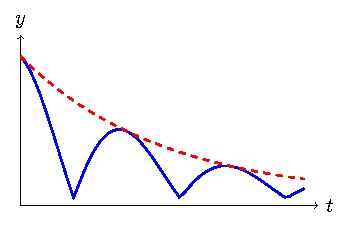
\includegraphics[width=0.6\linewidth]{signal}
  \caption{A damped signal (PDF figure).}
  \label{fig:signal}
\end{figure}

\begin{figure}[htbp]
  \centering
  \begin{subfigure}{0.45\textwidth}
    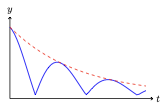
\includegraphics[width=\linewidth]{spectrum.png}
    \caption{PNG version}
    \label{fig:pair-a}
  \end{subfigure}
  \hfill
  \begin{subfigure}{0.45\textwidth}
    \includegraphics[width=\linewidth]{missing-figure}
    \caption{A missing file}
  \end{subfigure}
  \caption{Two views; panel~\ref{fig:pair-a} is a PNG.}
  \label{fig:pair}
\end{figure}

\subsection{Discussion}
\begin{itemize}
  \item Lists render with their items, including math like $\int_0^1 x\,dx = \tfrac12$.
  \item Theorem~\ref{thm:conv} is referenced by number.
  \item An undefined reference shows as \ref{sec:nowhere}.
\end{itemize}

\begin{enumerate}
  \item First numbered point.
  \item Second numbered point.
\end{enumerate}

% This comment is hidden in the output.
\bibliographystyle{plain}
\bibliography{refs}

\end{document}
